\section{Evaluation}
We evaluated the algorithms on multiple datasets (included with the code, in $data$ folder). We will present statistical data for two of them. We also ported the fixed grid filter and dynamic grid filter algorithms to Nao robot and did the practical demonstration.

In the first test ($test1$ in $data$ folder), we have one-dimensional state space. Initially, the sensor measurements have $3$ peaks. With time only one of the peaks survive. All the algorithms have around $100$ variables. We keep this fixed across algorithms to measure their relative performance. Using any other number of variables also gives similar results. (Except polynomial filter, due to lack of time, we could implement only up to degree $2$, so $3$ parameters only.)
\begin{itemize}
    \item Particle filter (PF): $100$ particles.
    \item Fixed grid filter (FGF): $100$ grid points.
    \item Dynamic grid filter (DGF): $50$ to $100$ grid points. (dynamic.)
    \item Neural network (NN): Two layers of size $10$. $10*10=100$. (approx.)
\end{itemize}

\begin{table}
\caption{Error in the state with maximum probability.}    
\begin{center}
\resizebox{\columnwidth}{!}{%
\begin{tabular}{ | c || c | c | c | c | c | }
Step & PF & FGF & DGF & PolyF & NN \\
1 & 0.7640 & 0.0640 & 7.8570 & 2.0640 & 4.5320 \\ 
2 & 0.0510 & 0.0620 & 0.6720 & 7.9380 & 2.7760 \\ 
3 & 0.0970 & 0.0600 & 2.3150 & 2.9910 & 2.9410 \\ 
4 & 0.4800 & 5.6930 & 0.0020 & 1.8340 & 0.9330 \\ 
5 & 0.5600 & 0.0390 & 1.8930 & 2.1310 & 1.6100 \\ 
6 & 0.1020 & 0.0270 & 1.1850 & 1.0340 & 1.0370 \\ 
7 & 0.2680 & 0.0330 & 0.2470 & 1.0580 & 0.8970 \\ 
8 & 0.5250 & 0.0160 & 0.1320 & 0.8490 & 0.0010 \\ 
9 & 0.2520 & 0.0230 & 0.1910 & 0.9160 & 0.3730 \\ 
10 & 0.0820 & 0.0290 & 0.1310 & 0.7960 & 0.4750 
\end{tabular}}
\end{center}
\end{table}

\begin{table}
\caption{Error in the mean of estimated state.}    
\begin{center}
\resizebox{\columnwidth}{!}{%
\begin{tabular}{ | c || c | c | c | c | c | }
Step & PF & FGF & DGF & PolyF & NN \\
1 & 0.5007 & 0.0010 & 0.1915 & 0.0224 & 0.0259 \\  
2 & 0.6320 & 0.0015 & 0.4271 & 0.2390 & 0.2663 \\  
3 & 0.3487 & 0.0018 & 0.7181 & 0.3715 & 0.4382 \\  
4 & 0.1031 & 0.0020 & 1.0043 & 0.5999 & 0.4570 \\  
5 & 0.3854 & 0.0021 & 1.2934 & 0.5197 & 0.2080 \\  
6 & 0.4882 & 0.0022 & 1.4082 & 0.0116 & 0.0971 \\  
7 & 0.4264 & 0.0023 & 1.3687 & 0.8871 & 1.0026 \\  
8 & 0.1852 & 0.0023 & 1.2192 & 1.8244 & 1.5367 \\  
9 & 0.0173 & 0.0023 & 1.0895 & 2.7725 & 2.1200 \\  
10 & 0.2027 & 0.0023 & 0.9733 & 3.5915 & 2.3507 
\end{tabular}}
\end{center}
\end{table}

\begin{table}
\caption{L2-error in computed CDF.}    
\begin{center}
\resizebox{\columnwidth}{!}{%
\begin{tabular}{ | c || c | c | c | c | c | }
Step & PF & FGF & DGF & PolyF & NN \\
1 & 5.5895 & 0.3385 & 5.6089 & 4.7394 & 5.5770 \\  
2 & 3.1485 & 0.3799 & 4.7029 & 7.9123 & 8.0532 \\  
3 & 5.1527 & 0.4117 & 5.0591 & 8.9555 & 8.0353 \\  
4 & 4.5226 & 0.4256 & 5.4113 & 9.6027 & 7.7276 \\  
5 & 9.2158 & 0.4360 & 6.1948 & 10.0842 & 8.2515 \\  
6 & 7.7962 & 0.4820 & 5.6106 & 13.5393 & 9.0468 \\  
7 & 7.1645 & 0.5667 & 4.6130 & 18.8865 & 14.8883 \\  
8 & 7.4783 & 0.6547 & 4.0991 & 21.6299 & 12.3882 \\  
9 & 5.9185 & 0.7172 & 3.4860 & 22.7425 & 12.8611 \\  
10 & 5.7165 & 0.7603 & 3.0654 & 22.6650 & 10.1677 
\end{tabular}}
\end{center}
\end{table}


\begin{figure}
\caption{Test 1. Cumulative Distribution Functions after $3$ time steps.}
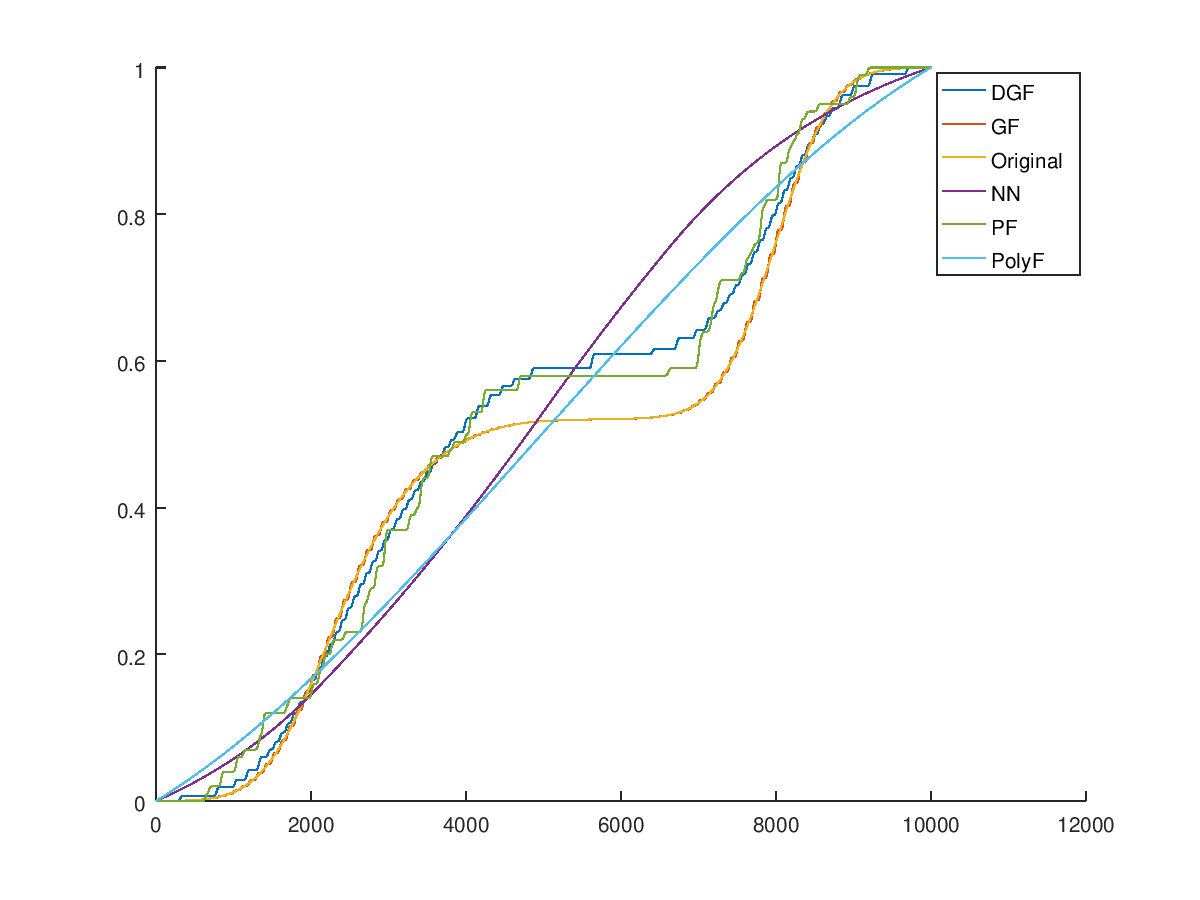
\includegraphics[width=\linewidth]{test1_03}
\end{figure}

\begin{figure}
\caption{Test 1. Cumulative Distribution Functions after $6$ time steps.}
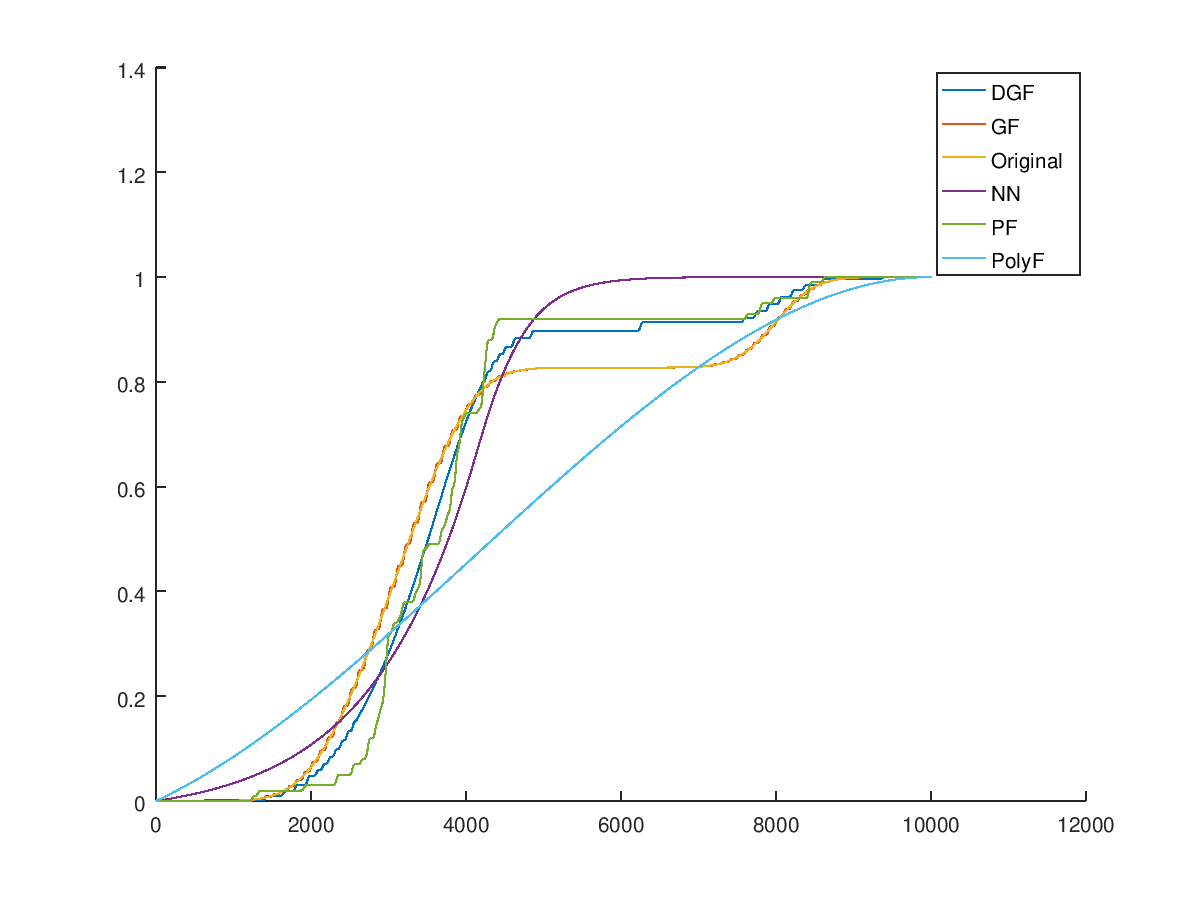
\includegraphics[width=\linewidth]{test1_06}
\end{figure}

\begin{figure}
\caption{Test 1. Cumulative Distribution Functions after $10$ time steps.}
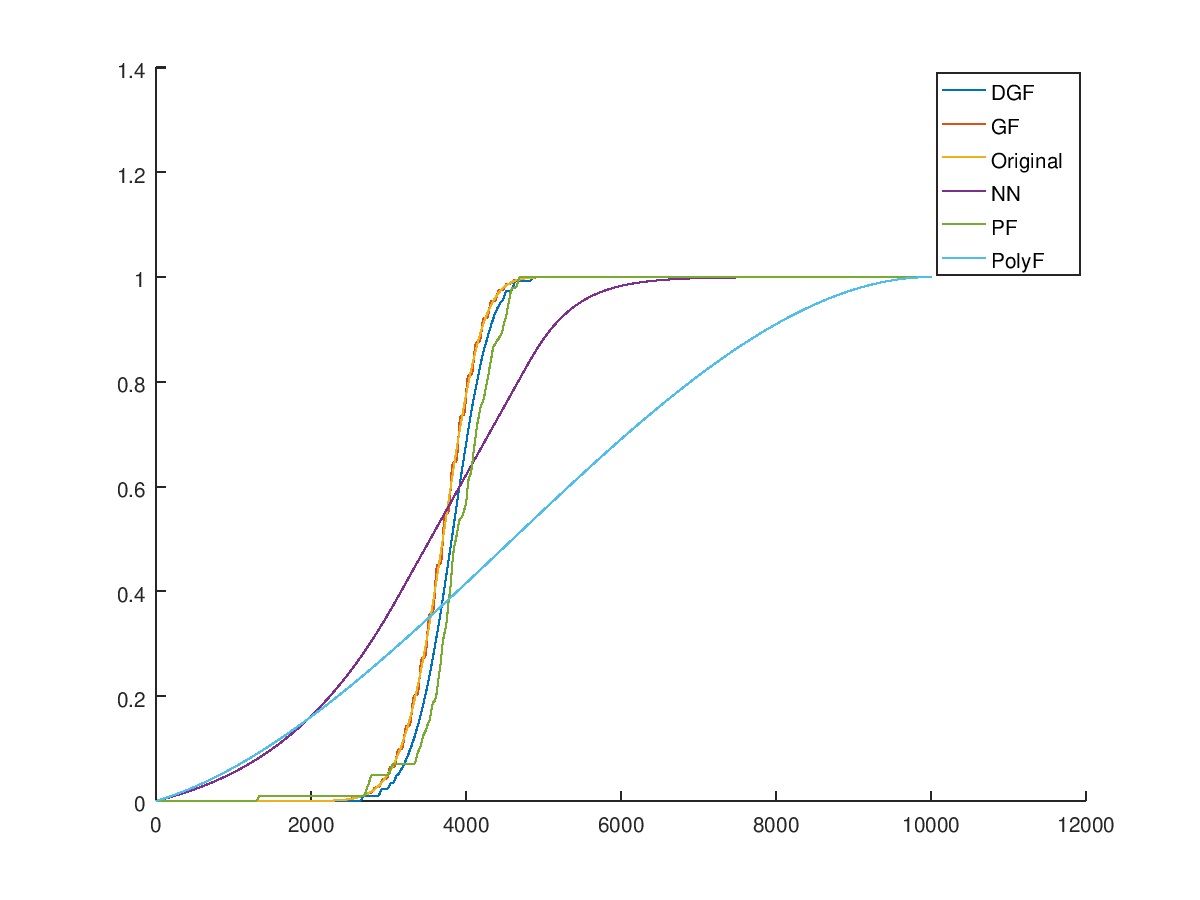
\includegraphics[width=\linewidth]{test1_10}
\end{figure}

In the second test ($test3$ in $data$ folder), we have multi-dimensional state space. Here also, all the algorithms have around $100$ parameters.
\begin{itemize}
    \item Particle filter (PF): $100$ particles.
    \item Fixed grid filter (FGF): $100$ grid points.
    \item Dynamic grid filter (DGF): $50$ to $100$ grid points. (dynamic.)
    \item Neural network (NN): Two layers of size $10$. $10*10=100$. (approx.)
\end{itemize}

\begin{table}
\caption{Error in the state with maximum probability.}    
\begin{center}
\resizebox{\columnwidth}{!}{%
\begin{tabular}{ | c || c | c | c | c | c | }
Step & PF & FGF & DGF & PolyF & NN \\
1 & 73.5391 & 85.7030 & 87.8465 & 74.4648 \\ 
2 & 72.0139 & 4.0000 & 72.0069 & 84.4808 & 80.2808 \\ 
3 & 81.0247 & 35.8469 & 21.4709 & 19.0263 & 85.0706 \\ 
4 & 51.4782 & 1.0000 & 64.4127 & 111.3598 \\ 
5 & 76.0592 & 50.2494 & 2.0000 & 48.7647 & 109.6586 \\ 
6 & 1.0000 & 40.3113 & 53.8516 & 109.6586 \\ 
7 & 74.6860 & 28.1603 & 54.7449 & 47.6760 & 110.4943 \\ 
8 & 75.1532 & 19.4165 & 57.8705 & 48.0416 & 110.0727 \\ 
9 & 42.0595 & 26.9258 & 4.4721 & 6.3246 & 56.8595 \\ 
10 & 20.5913 & 32.9848 & 1.4142 & 7.0711 & 58.5235
\end{tabular}}
\end{center}
\end{table}

\begin{table}
\caption{Error in the mean of estimated state.}    
\begin{center}
\resizebox{\columnwidth}{!}{%
\begin{tabular}{ | c || c | c | c | c | c | }
Step & PF & FGF & DGF & PolyF & NN \\
1 & 20.3808 & 15.3506 & 8.1420 & 13.7211 & 63.1493 \\ 
2 & 36.8619 & 36.3728 & 17.3435 & 30.9885 & 128.6551 \\ 
3 & 43.8748 & 40.6532 & 18.4665 & 38.5199 & 195.4936 \\ 
4 & 20.8605 & 70.5275 & 16.4776 & 43.2564 & 267.7114 \\ 
5 & 22.3279 & 108.4227 & 24.0023 & 62.1079 & 344.1171 \\ 
6 & 62.2529 & 138.1839 & 50.4984 & 95.0064 & 422.2877 \\ 
7 & 112.1986 & 149.7854 & 82.5249 & 126.4093 & 496.9704 \\ 
8 & 165.0571 & 149.9109 & 115.0814 & 156.5516 & 569.8333 \\ 
9 & 197.9973 & 125.5558 & 115.3565 & 151.7752 & 611.9340 \\ 
10 & 205.5056 & 93.5752 & 113.8170 & 149.8863 & 654.5354
\end{tabular}}
\end{center}
\end{table}

\begin{table}
\caption{L2-error in computed CDF.}    
\begin{center}
\resizebox{\columnwidth}{!}{%
\begin{tabular}{ | c || c | c | c | c | c | }
Step & PF & FGF & DGF & PolyF & NN \\
1 & 7.6426 & 10.2127 & 9.9363 & 11.2119 & 32.0021 \\ 
2 & 10.5246 & 14.1116 & 11.6408 & 15.4432 & 51.6483 \\ 
3 & 5.9152 & 23.5160 & 1.9137 & 10.3824 & 63.1219 \\ 
4 & 12.5345 & 15.8151 & 2.9442 & 11.9974 & 56.4408 \\ 
5 & 25.6487 & 7.7291 & 5.7329 & 16.4528 & 46.7826 \\ 
6 & 24.7311 & 6.4264 & 5.8499 & 17.4547 & 46.0956 \\ 
7 & 32.6005 & 5.0391 & 5.9658 & 14.7962 & 50.0060 \\ 
8 & 37.1039 & 7.5916 & 10.7382 & 13.6126 & 47.1922 \\ 
9 & 47.8120 & 19.3311 & 9.7274 & 19.8916 & 26.0166 \\ 
10 & 13.7839 & 11.4408 & 4.3487 & 20.5015 & 25.8191
\end{tabular}}
\end{center}
\end{table}

In these experiments, we observed that NN and PolyF severely underperformed. Also, using appropriate hyper-parameters for the NNs can improve the performance significantly.

In the first test, the FGF performed better than the PF. The PF and the DGF performed comparably. In the second test, the FGF was worse than PF and DGF. In all these tests, although the DGF and PF have the same number of parameters, DGF takes much more processing time than PF. This makes using DGF in Nao much slower.